\chapter{Fluid Kinematics}\label{ch:b2:fluid-kinematics}

Stand on a bridge and watch the river. A leaf drifts past, speeds up
between the piers, slows in the pool below, circles once in an eddy and
moves on. You could describe the river by following that leaf --- its
position and velocity at every instant --- or by standing still and
recording, at every point of the river, how fast the water passes. The
second description is the fluid physicist's: a \emph{velocity field}.
This chapter sets up the two descriptions, learns to compute the
acceleration of a particle from the field, writes the conservation of
mass as a local law, and classifies flows by whether they swirl --- the
vocabulary that Euler's and Navier's equations will need.

\begin{omfigure}
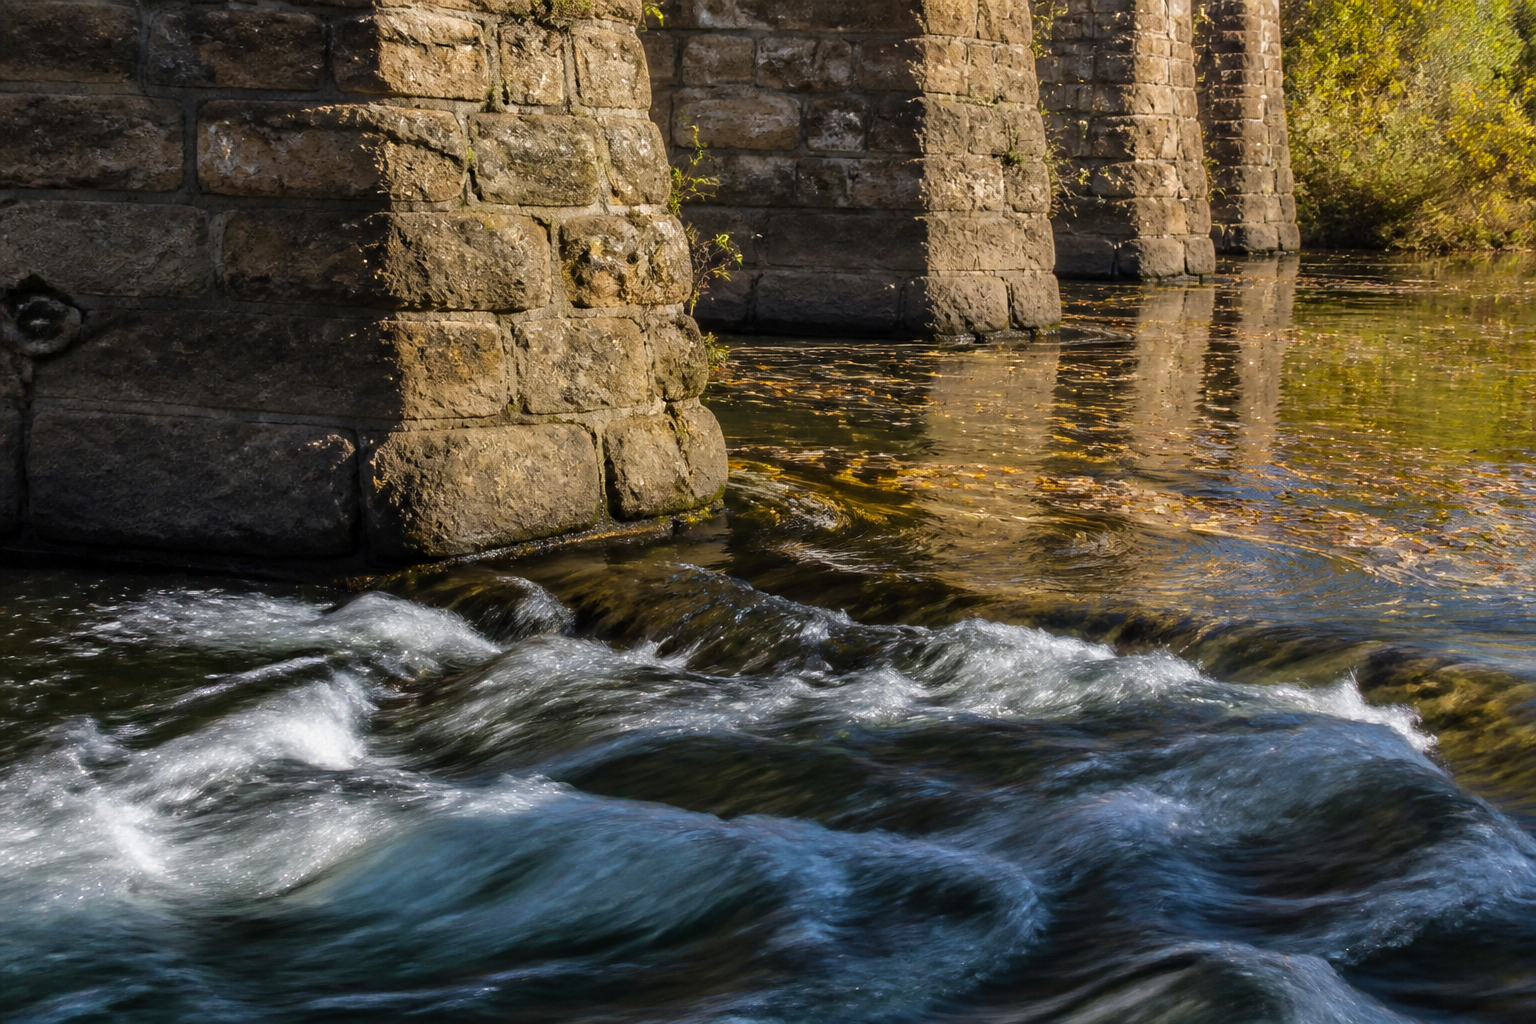
\includegraphics[width=0.58\linewidth]{images/book4/ai/b4-02-river-bridge-eddies.png}

{\small A river past a bridge: fast, smooth water between the piers, eddies in their lee --- a velocity field to be read at fixed points, not a single trajectory to be followed.}
\end{omfigure}


\section{The continuum description}

\begin{definition}[Fluid particle; the continuum hypothesis]\label{def:b2:fluid-kinematics:particle}
\index{fluid particle}\index{continuum hypothesis}\index{mesoscopic scale}
A \emph{fluid particle} is a volume of fluid small enough to be treated
as a point on the scale of the flow, yet large enough to contain a huge
number of molecules, so that its density $\rho$, pressure $P$,
temperature $T$ and mean velocity $\vect v$ are well-defined averages
(the \emph{mesoscopic} scale, typically a micrometre). The \emph{continuum
hypothesis} assumes such a scale exists: the mean free path $\ell$ of
the molecules must be much smaller than the scale $L$ of the flow,
$\ell/L \ll 1$. In air at atmospheric pressure $\ell \approx \qty{70}{nm}$; in
a liquid $\ell$ is the molecular size. The fluid is then described by
\emph{fields} $\rho(M, t)$, $P(M, t)$, $\vect v(M, t)$ defined at every point.
\end{definition}

\begin{definition}[Lagrangian and Eulerian descriptions]\label{def:b2:fluid-kinematics:euler}
\index{Lagrangian description}\index{Eulerian description}\index{streamline}\index{pathline}\index{stationary flow}
The \emph{Lagrangian} description follows each \omterm{def:b2:fluid-kinematics:particle}{fluid particle}: its
position $\vect r(t)$ and velocity $\dd\vect r/\dd t$ as functions of time
and of its initial position. The \emph{Eulerian} description gives, at
each fixed point $M$ and time $t$, the velocity $\vect v(M, t)$ of the
particle that is passing through $M$ at that instant. A \emph{pathline}
is the trajectory of a particle; a \emph{streamline} at time $t$ is a
curve tangent at every point to $\vect v(M, t)$; a \emph{stream tube} is
the surface made of the streamlines through a closed curve. A flow is
\emph{stationary} (steady) when the Eulerian fields do not depend on
time, $\partial\vect v/\partial t = \vect 0$; then streamlines and pathlines
coincide and are fixed.
\end{definition}

\begin{example}[Two descriptions of one flow]\label{ex:b2:fluid-kinematics:hose}
Water in a garden hose of section $S$ at flow rate $Q$ moves at $v = Q/S$
everywhere: the Eulerian field is uniform and the Lagrangian motion of
each particle is uniform. In the tapering nozzle the Eulerian field is
still steady but $v$ increases along the axis: every particle
\emph{accelerates} as it passes through, though nothing at any fixed
point changes with time. That is the first thing the \omterm{def:b2:fluid-kinematics:euler}{Eulerian
description} must learn to express.
\end{example}

\begin{omfigure}
\begin{tikzpicture}[font=\small, x=1cm, y=1cm, >=Stealth]
  \begin{scope}
    % streamlines of a converging channel
    \foreach \y in {-1.2,-0.6,0,0.6} {
      \draw[omDef, thick, postaction={decorate, decoration={markings, mark=at position 0.55 with {\arrow{>}}}}]
        (-2.8,\y) .. controls (-0.8,\y) and (0.2,{0.45*\y}) .. (2.8,{0.45*\y});
    }
    \draw[omDef, thick, postaction={decorate, decoration={markings, mark=at position 0.55 with {\arrow{>}}}}]
        (-2.8,1.2) .. controls (-0.8,1.2) and (0.2,0.54) .. (2.8,0.54)
        coordinate[pos=0.15] (P1) coordinate[pos=0.6] (P2) coordinate[pos=0.9] (P3);
    \draw[thick] (-2.8,1.6) .. controls (-0.8,1.6) and (0.2,0.75) .. (2.8,0.75);
    \draw[thick] (-2.8,-1.6) .. controls (-0.8,-1.6) and (0.2,-0.75) .. (2.8,-0.75);
    \fill[omThm] (P1) circle (2pt) node[above, font=\footnotesize, yshift=1pt] {$t_1$};
    \fill[omThm] (P2) circle (2pt) node[above, font=\footnotesize, yshift=1pt] {$t_2$};
    \fill[omThm] (P3) circle (2pt) node[above, font=\footnotesize, yshift=1pt] {$t_3$};
    \node[font=\footnotesize, align=center] at (0,-2.15) {steady flow: streamlines $=$ pathlines,\\a particle speeds up where the tube narrows};
  \end{scope}
  \begin{scope}[xshift=7.4cm]
    \draw[thick,->] (-2.8,-1.2) -- (2.8,-1.2) node[right, font=\footnotesize] {$x$};
    \draw[thick,->] (-2.8,-1.2) -- (-2.8,1.6);
    % velocity vectors at fixed points (Eulerian)
    \foreach \x in {-2.2,-1.2,-0.2,0.8,1.8} \foreach \y in {-0.6,0.2,1.0} {
      \draw[omDef, ->] (\x,\y) -- ({\x+0.5+0.12*\x},{\y+0.15*\y});
    }
    \node[omDef, font=\footnotesize] at (0,1.75) {Eulerian: $\vect v(M,t)$ at fixed points};
    \draw[omThm, thick, ->] (-2.5,-0.9) .. controls (-1,-0.3) and (0.5,0.9) .. (2.4,1.3);
    \node[omThm, font=\footnotesize] at (2.2,0.7) {pathline};
    \node[font=\footnotesize, align=center] at (0,-1.95) {Lagrangian: follow one particle};
  \end{scope}
\end{tikzpicture}

{\small Left: a steady converging flow --- the \omterm{def:b2:fluid-kinematics:euler}{streamlines} are fixed,
a marked particle follows one of them and accelerates as the tube
narrows. Right: the \omterm{def:b2:fluid-kinematics:euler}{Eulerian description} records the velocity vector
at fixed points; the Lagrangian one follows a particle along its
\omterm{def:b2:fluid-kinematics:euler}{pathline}.}
\end{omfigure}

\section{The material derivative}

\begin{theorem}[Material (particle) derivative]\label{thm:b2:fluid-kinematics:material}
\index{material derivative}\index{convective acceleration}
The rate of change of a quantity $G(M, t)$ (scalar or vector) \emph{for
the \omterm{def:b2:fluid-kinematics:particle}{fluid particle}} passing through $M$ at time $t$ is
\[
\frac{\mathrm DG}{\mathrm Dt} = \frac{\partial G}{\partial t} + (\vect v\cdot
\operatorname{\vect{grad}})\,G ,
\qquad\text{in particular}\qquad
\vect a = \frac{\mathrm D\vect v}{\mathrm Dt} = \frac{\partial\vect v}{\partial t} +
(\vect v\cdot\operatorname{\vect{grad}})\,\vect v ,
\]
where $(\vect v\cdot\operatorname{\vect{grad}}) = v_x\partial_x + v_y\partial_y +
v_z\partial_z$. The first term is the \emph{local} rate of change (at a
fixed point), the second the \emph{convective} one (because the particle
moves to where $G$ is different). For the velocity, $(\vect v\cdot
\operatorname{\vect{grad}})\vect v = \operatorname{\vect{grad}}(v^2/2) +
(\operatorname{\vect{curl}}\vect v)\wedge\vect v$.
\end{theorem}

\begin{proof}
In $\dd t$ the particle moves from $M$ to $M + \vect v\,\dd t$, so $\dd G =
G(M + \vect v\dd t, t + \dd t) - G(M, t) = \partial_tG\,\dd t + \dd t\,(v_x\partial_x
+ v_y\partial_y + v_z\partial_z)G$ to first order (chain rule for a function
of four variables). The vector identity is checked on the $x$
component: $[\operatorname{\vect{grad}}(v^2/2)]_x = v_x\partial_xv_x + v_y\partial_x
v_y + v_z\partial_xv_z$ and $[(\operatorname{\vect{curl}}\vect v)\wedge\vect v]_x =
v_y(\partial_yv_x - \partial_xv_y) + v_z(\partial_zv_x - \partial_xv_z)$ (with the
components of $\operatorname{\vect{curl}}\vect v$ given below in
\cref{def:b2:fluid-kinematics:vorticity}); their sum is $v_x\partial_xv_x +
v_y\partial_yv_x + v_z\partial_zv_x$.
\end{proof}

\begin{example}[Acceleration in a steady nozzle]\label{ex:b2:fluid-kinematics:nozzle}
A one-dimensional steady flow $v(x) = v_0(1 + x/L)$ along a nozzle: the
local term vanishes, and $a = v\,\dd v/\dd x = v_0^2(1 + x/L)/L$. A
particle that enters at $v_0 = \qty{2}{m/s}$ and leaves at $2v_0$ over $L
= \qty{5}{cm}$ feels $a = 80$ to \qty{160}{m/s^2}: eight to sixteen $g$, in a
flow where nothing depends on time.
\end{example}

\begin{example}[Local versus convective]\label{ex:b2:fluid-kinematics:weather}
Temperature at a weather station falls during the night ($\partial T/
\partial t < 0$: local), and falls for an air parcel carried northward by
the wind ($\vect v\cdot\operatorname{\vect{grad}}T < 0$: convective, or
\emph{advective}). A thermometer on a balloon drifting with the wind
records the sum, $\mathrm DT/\mathrm Dt$; the weather station records only
the first term.
\end{example}

\section{Conservation of mass}

\begin{definition}[Mass flow rate and volume flow rate]\label{def:b2:fluid-kinematics:flowrate}
\index{mass flow rate}\index{volume flow rate}\index{mass flux}
The \emph{mass flow rate} through an oriented surface $S$ is the mass
crossing it per unit time, $D_m = \sum\rho\,\vect v\cdot\vect n\,\dd S$ ---
the flux of the \emph{mass current density} $\vect j = \rho\vect v$ (unit
\unit{kg.m^{-2}.s^{-1}}); the \emph{volume flow rate} is $D_V = \sum\vect v
\cdot\vect n\,\dd S$ (\unit{m^3/s}). For a uniform velocity normal to a plane
section of area $S$, $D_m = \rho vS$ and $D_V = vS$.
\end{definition}

\begin{proof}
In $\dd t$ the fluid crossing the element $\dd S$ is that contained in
the oblique cylinder of base $\dd S$ and generator $\vect v\,\dd t$, of
volume $\vect v\cdot\vect n\,\dd S\,\dd t$ and mass $\rho$ times that.
\end{proof}

\begin{theorem}[Local conservation of mass]\label{thm:b2:fluid-kinematics:continuity}
\index{continuity equation}\index{divergence}
At every point of a fluid,
\[
\frac{\partial\rho}{\partial t} + \operatorname{div}(\rho\vect v) = 0 ,
\qquad\text{where}\qquad
\operatorname{div}\vect A = \frac{\partial A_x}{\partial x} + \frac{\partial A_y}{\partial y} +
\frac{\partial A_z}{\partial z}
\]
is the \emph{divergence} of a vector field: the net outgoing flux of
$\vect A$ through the surface of a small volume, per unit volume.
Equivalently $\mathrm D\rho/\mathrm Dt + \rho\operatorname{div}\vect v = 0$.
\end{theorem}

\begin{proof}
Take the fixed box $[x, x + \dd x]\times[y, y + \dd y]\times[z, z + \dd z]$.
Its mass $\rho\,\dd x\dd y\dd z$ changes at the rate $\partial_t\rho\,\dd x\dd y
\dd z$. Mass enters through the face at $x$ at the rate $j_x(x)\dd y\dd z$
and leaves through the face at $x + \dd x$ at $j_x(x + \dd x)\dd y\dd z$:
net outflow $\partial_xj_x\,\dd x\dd y\dd z$, and likewise for $y$ and $z$.
Conservation of mass --- no mass is created --- gives $\partial_t\rho = -
(\partial_xj_x + \partial_yj_y + \partial_zj_z)$. The second form follows from
$\operatorname{div}(\rho\vect v) = \vect v\cdot\operatorname{\vect{grad}}\rho +
\rho\operatorname{div}\vect v$.
\end{proof}

\begin{remark}[The divergence, a first meeting]\label{rem:b2:fluid-kinematics:divergence}
The derivation shows what $\operatorname{div}$ measures: the flux leaving
a small box per unit volume. Summing over the boxes that tile a finite
volume $V$, the interior faces cancel pairwise and only the outer
surface remains: $\iint_{\partial V}\vect A\cdot\vect n\,\dd S = \iiint_V
\operatorname{div}\vect A\,\dd\tau$ --- the divergence (Ostrogradski)
theorem, which we shall state properly in \cref{ch:b2:maxwell-equations}
and use throughout electromagnetism; it is proved in the Year 3
mathematics volume. Integrated over a fixed volume, the local law reads
$\dd m_V/\dd t = -D_m^{\text{out}}$: the mass inside changes by what
crosses the boundary.
\end{remark}

\begin{omfigure}
\begin{tikzpicture}[font=\small, x=1cm, y=1cm, >=Stealth]
  \begin{scope}
    \draw[thick, fill=omDef!10] (0,0) rectangle (2.2,1.6);
    \draw[thick] (0,1.6) -- (0.6,2.1) -- (2.8,2.1) -- (2.2,1.6);
    \draw[thick] (2.2,0) -- (2.8,0.5) -- (2.8,2.1);
    \draw[omThm, very thick, ->] (-1.2,0.8) -- (-0.1,0.8) node[pos=0.3, above, font=\footnotesize] {$j_x(x)$};
    \draw[omThm, very thick, ->] (2.3,0.8) -- (3.6,0.8) node[pos=0.75, above, font=\footnotesize] {$j_x(x+\dd x)$};
    \node[font=\footnotesize] at (1.1,-0.35) {$\dd x$};
    \node[font=\footnotesize] at (-0.35,0.3) {$\dd y$};
    \node[font=\footnotesize] at (2.75,-0.05) {$\dd z$};
    \node[font=\footnotesize, align=left] at (1.3,-1.1) {$\partial_t\rho\,\dd\tau = -(\partial_x j_x + \partial_y j_y + \partial_z j_z)\,\dd\tau$};
  \end{scope}
  \begin{scope}[xshift=8.2cm]
    \draw[thick] (-2.4,1.1) .. controls (-1,1.1) and (0,0.5) .. (2.4,0.5);
    \draw[thick] (-2.4,-1.1) .. controls (-1,-1.1) and (0,-0.5) .. (2.4,-0.5);
    \draw[omDef, thick] (-2.4,0) ellipse (0.25 and 1.1);
    \draw[omDef, thick] (2.4,0) ellipse (0.12 and 0.5);
    \draw[omThm, very thick, ->] (-2.4,0) -- (-1.4,0) node[above, font=\footnotesize] {$v_1$};
    \draw[omThm, very thick, ->] (2.4,0) -- (3.6,0) node[above, font=\footnotesize] {$v_2$};
    \node[omDef, font=\footnotesize] at (-2.4,1.45) {$S_1$};
    \node[omDef, font=\footnotesize] at (2.4,0.85) {$S_2$};
    \node[font=\footnotesize] at (0,-1.6) {steady: $\rho_1v_1S_1 = \rho_2v_2S_2$};
  \end{scope}
\end{tikzpicture}

{\small Left: the mass balance of a fixed box --- the net outflow
through its six faces, per unit volume, is the divergence of $\rho\vect v$.
Right: in a steady flow the \omterm{def:b2:fluid-kinematics:flowrate}{mass flow rate} is the same through every
section of a stream tube.}
\end{omfigure}

\begin{corollary}[Incompressible flow; stream tubes]\label{cor:b2:fluid-kinematics:incompressible}
\index{incompressible flow}
A flow is \emph{incompressible} when the density of each particle stays
constant, $\mathrm D\rho/\mathrm Dt = 0$, which is equivalent to
\[
\operatorname{div}\vect v = 0 .
\]
A homogeneous liquid flows incompressibly; so does a gas at speeds well
below the speed of sound (see \cref{ch:b2:sound-waves}). In a steady
flow the \omterm{def:b2:fluid-kinematics:flowrate}{mass flow rate} $\rho vS$ is the same through every section of
a stream tube; if moreover the flow is incompressible and $\rho$ uniform,
$vS$ is constant: the fluid speeds up where the tube narrows.
\end{corollary}

\begin{proof}
$\mathrm D\rho/\mathrm Dt = -\rho\operatorname{div}\vect v$. For the tube,
apply the integrated balance to the volume between two sections: no
flux through the lateral surface (velocity tangent), steady state, so
inflow equals outflow.
\end{proof}

\begin{example}[Blood]\label{ex:b2:fluid-kinematics:blood}
The aorta (section \qty{2.5}{cm^2}) carries \qty{5}{L/min} $= \qty{83}{cm^3/s}$:
$v = \qty{33}{cm/s}$. The same flow passes through some $10^{10}$
capillaries of total section about \qty{2500}{cm^2}: $v = \qty{0.3}{mm/s}$ ---
slow enough for exchanges through the walls, the point of the branching.
\end{example}

\section{Vorticity and irrotational flows}

\begin{definition}[Vorticity]\label{def:b2:fluid-kinematics:vorticity}
\index{vorticity}\index{curl}\index{irrotational flow}
The \emph{vorticity} of a flow is the vector field
\[
\vect\omega = \operatorname{\vect{curl}}\vect v , \qquad
\operatorname{\vect{curl}}\vect A = \Bigl(\frac{\partial A_z}{\partial y} -
\frac{\partial A_y}{\partial z},\; \frac{\partial A_x}{\partial z} - \frac{\partial A_z}
{\partial x},\; \frac{\partial A_y}{\partial x} - \frac{\partial A_x}{\partial y}\Bigr) .
\]
A flow is \emph{irrotational} where $\vect\omega = \vect 0$.
\end{definition}

\begin{proposition}[Vorticity measures local rotation]\label{prop:b2:fluid-kinematics:rotation}
A small fluid element centred at $M$ rotates, as a whole, with the
angular velocity $\vect\Omega = \tfrac12\vect\omega(M)$. In a solid-body
rotation $\vect v = \vect\Omega\wedge\vect{OM}$ the \omterm{def:b2:fluid-kinematics:vorticity}{vorticity} is uniform,
$\vect\omega = 2\vect\Omega$; in the plane shear flow $\vect v = ky\,\vect e_x$
it is $\vect\omega = -k\vect e_z$: a paddle wheel dropped in a shear flow
turns although the \omterm{def:b2:fluid-kinematics:euler}{streamlines} are straight.
\end{proposition}

\begin{proof}
Near $M$, $\vect v(M + \vect\epsilon) = \vect v(M) + \mathbf G\vect\epsilon$ with
$\mathbf G$ the matrix of $\partial_jv_i$; split it into its symmetric part
(a pure strain, which stretches the element without turning it as a
whole) and its antisymmetric part, whose matrix $\tfrac12(\partial_jv_i -
\partial_iv_j)$ is that of $\vect\epsilon \mapsto \tfrac12\vect\omega\wedge\vect\epsilon$
(\cref{thm:b2:rigid-body-mechanics:field}). Solid rotation about $\vect e_z$:
$\vect v = \Omega(-y, x, 0)$, $\omega_z = \partial_xv_y - \partial_yv_x = 2\Omega$.
Shear: $\omega_z = -\partial_y(ky) = -k$.
\end{proof}

\begin{definition}[Velocity potential; circulation]\label{def:b2:fluid-kinematics:potential}
\index{velocity potential}\index{circulation (of velocity)}\index{potential flow}
In an \omterm{def:b2:fluid-kinematics:vorticity}{irrotational flow} the velocity derives from a \emph{velocity
potential}: $\vect v = \operatorname{\vect{grad}}\varphi$ (the circulation
of $\vect v$ along a path then depends only on its ends, $\int_A^B\vect v
\cdot\dd\vect l = \varphi(B) - \varphi(A)$). If the flow is also
incompressible, $\Delta\varphi = \operatorname{div}\operatorname{\vect{grad}}
\varphi = 0$: the potential obeys Laplace's equation, exactly like the
electrostatic potential in a charge-free region --- a \emph{potential
flow}. The \emph{circulation} of the velocity along a closed curve $C$
is $\Gamma = \oint_C\vect v\cdot\dd\vect l$.
\end{definition}

\begin{proof}
That a curl-free field on a simply connected region is a gradient, and
that a gradient is curl-free ($\partial_y\partial_z\varphi = \partial_z\partial_y\varphi$),
are the Year 2 mathematics volume's; Laplace's equation follows from
$\operatorname{div}\vect v = 0$.
\end{proof}

\begin{example}[Three plane flows]\label{ex:b2:fluid-kinematics:planeflows}
\index{stagnation flow}\index{point vortex}\index{Rankine vortex}
(i) \emph{\omterm{ex:b2:fluid-kinematics:planeflows}{Stagnation flow}} $\vect v = k(x, -y)$: $\operatorname{div}\vect v =
0$, $\vect\omega = \vect 0$, $\varphi = \tfrac12k(x^2 - y^2)$; \omterm{def:b2:fluid-kinematics:euler}{streamlines}
$xy = $ const, hyperbolas --- a jet hitting a wall, near the axis. (ii)
\emph{\omterm{ex:b2:fluid-kinematics:planeflows}{Point vortex}} $\vect v = \dfrac{\Gamma}{2\pi r}\vect e_\theta$ (plane
polar coordinates): incompressible and \emph{irrotational everywhere
except at $r = 0$}, $\varphi = \Gamma\theta/2\pi$ (multivalued), and the
circulation on any circle around the centre is $\Gamma$ --- the
\omterm{def:b2:fluid-kinematics:vorticity}{vorticity} is concentrated on the axis. (iii) \emph{\omterm{ex:b2:fluid-kinematics:planeflows}{Rankine vortex}}: a
core $r < a$ in solid rotation $v_\theta = \Omega r$ (\omterm{def:b2:fluid-kinematics:vorticity}{vorticity} $2\Omega$)
matched to the \omterm{ex:b2:fluid-kinematics:planeflows}{point vortex} $v_\theta = \Omega a^2/r$ outside: the model of
a tornado, a bathtub swirl or the eddy behind the bridge pier --- the
velocity peaks at the edge of the core.
\end{example}

\begin{omfigure}
\begin{tikzpicture}[font=\small, x=1cm, y=1cm, >=Stealth]
  \begin{scope}
    \foreach \c in {0.3,0.8,1.6,2.8} {
      \draw[omDef, thick, domain={\c/2.4}:2.4, samples=40, postaction={decorate, decoration={markings, mark=at position 0.5 with {\arrow{>}}}}] plot (\x,{\c/\x});
      \draw[omDef, thick, domain=-2.4:{-\c/2.4}, samples=40, postaction={decorate, decoration={markings, mark=at position 0.5 with {\arrow{<}}}}] plot (\x,{-\c/\x});
    }
    \draw[thick] (-2.5,0) -- (2.5,0);
    \draw[->] (0,0) -- (0,2.6) node[right, font=\footnotesize] {$y$};
    \node[font=\footnotesize] at (0,-0.4) {stagnation flow $\vect v = k(x,-y)$};
  \end{scope}
  \begin{scope}[xshift=6.6cm]
    \foreach \r in {0.5,0.9,1.3,1.7} \draw[omDef, thick, postaction={decorate, decoration={markings, mark=at position 0.25 with {\arrow{>}}}}] (0,0) circle (\r);
    \fill (0,0) circle (1.5pt);
    \node[font=\footnotesize] at (0,-2.2) {point vortex $v_\theta = \Gamma/2\pi r$};
  \end{scope}
  \begin{scope}[xshift=10.6cm]
    \begin{axis}[omaxis, axis x line=bottom, axis y line=left, width=4.4cm, height=3.9cm, at={(0,-1.9cm)},
        xlabel={$r/a$}, ylabel={$v_\theta$}, xmin=0, xmax=4, ymin=0, ymax=1.2, xtick={1,2,3}, ytick=\empty,
        xlabel style={at={(axis description cs:0.5,-0.12)}, anchor=north},
        ylabel style={at={(axis description cs:-0.08,0.5)}, rotate=90, anchor=south}, samples=60]
      \addplot[omThm, thick, domain=0:1] {x};
      \addplot[omThm, thick, domain=1:4] {1/x};
      \node[font=\scriptsize] at (axis cs:0.55,0.85) {$\Omega r$};
      \node[font=\scriptsize] at (axis cs:2.6,0.62) {$\Omega a^2/r$};
    \end{axis}
  \end{scope}
\end{tikzpicture}

{\small Three plane flows. Left: the \omterm{ex:b2:fluid-kinematics:planeflows}{stagnation flow}, irrotational,
with hyperbolic \omterm{def:b2:fluid-kinematics:euler}{streamlines}. Middle: the \omterm{ex:b2:fluid-kinematics:planeflows}{point vortex} --- circular
\omterm{def:b2:fluid-kinematics:euler}{streamlines}, yet zero \omterm{def:b2:fluid-kinematics:vorticity}{vorticity} away from the centre. Right: the
\omterm{ex:b2:fluid-kinematics:planeflows}{Rankine vortex} profile, solid rotation in the core and a \omterm{ex:b2:fluid-kinematics:planeflows}{point vortex}
outside.}
\end{omfigure}

\begin{remark}[Why the circulation matters]\label{rem:b2:fluid-kinematics:stokes}
For a small plane loop of area $\dd S$ with normal $\vect n$, the
circulation is $\oint\vect v\cdot\dd\vect l = \vect\omega\cdot\vect n\,\dd S$ ---
the \omterm{def:b2:fluid-kinematics:vorticity}{vorticity} is the circulation per unit area, exactly as the
divergence is the flux per unit volume. (Check it on the solid-body
rotation: $2\pi r\cdot\Omega r = 2\Omega\cdot\pi r^2$.) Summed over a surface,
this gives Stokes' theorem, $\oint_C\vect v\cdot\dd\vect l = \iint_S
\operatorname{\vect{curl}}\vect v\cdot\vect n\,\dd S$, stated in
\cref{ch:b2:maxwell-equations}. A wing generates lift by carrying a
circulation around itself; a vortex line persists in a perfect fluid
(Kelvin's theorem) --- which is why the eddy behind the pier survives
so long.
\end{remark}

\begin{method}[Reading a velocity field]\label{met:b2:fluid-kinematics:reading}
Given $\vect v(M, t)$: (1) is it steady? ($\partial_t\vect v = \vect 0$); (2)
is it incompressible? ($\operatorname{div}\vect v = 0$); (3) is it
irrotational? ($\operatorname{\vect{curl}}\vect v = \vect 0$; if so find
$\varphi$); (4) find the \omterm{def:b2:fluid-kinematics:euler}{streamlines} from $\dd x/v_x = \dd y/v_y = \dd z/
v_z$ at fixed $t$, and the \omterm{def:b2:fluid-kinematics:euler}{pathlines} from $\dd\vect r/\dd t = \vect v(\vect r,
t)$; (5) compute the acceleration $\partial_t\vect v + (\vect v\cdot
\operatorname{\vect{grad}})\vect v$. In plane polar coordinates $(r, \theta)$,
$\operatorname{div}\vect v = \dfrac1r\dfrac{\partial(rv_r)}{\partial r} + \dfrac1r
\dfrac{\partial v_\theta}{\partial\theta}$ and $\omega_z = \dfrac1r\dfrac{\partial(rv_\theta)}
{\partial r} - \dfrac1r\dfrac{\partial v_r}{\partial\theta}$ (admitted here; derived
in \cref{ch:b2:maxwell-equations}).
\end{method}

\section{Exercises}

\begin{exercise}[$\star$]\label{exo:b2:fluid-kinematics:1}
The mean free path of air is \qty{70}{nm} at \qty{1}{bar} and varies as
$1/P$. Is the continuum description valid for (a) air around a car,
(b) air in a \qty{1}{\micro m} microchannel at \qty{1}{bar}, (c) air at
\qty{100}{km} altitude ($P \approx \qty{3e-7}{bar}$) around a \qty{1}{m}
satellite? Give $\ell/L$ in each case.
\end{exercise}

\begin{exercise}[$\star$]\label{exo:b2:fluid-kinematics:2}
Steady one-dimensional flow $v(x) = v_0(1 + x/L)$ for $0 \le x \le L$.
Acceleration of a particle at $x$; time it takes to cross from $0$ to
$L$; compare with $L/v_0$ and $L/2v_0$.
\end{exercise}

\begin{exercise}[$\star$]\label{exo:b2:fluid-kinematics:3}
In a pipe of radius $R$ the velocity profile is $v(r) = v_{\max}(1 -
r^2/R^2)$ along the axis. \omterm{def:b2:fluid-kinematics:flowrate}{Volume flow rate}; mean speed $\langle v\rangle
= D_V/\pi R^2$; numbers for $R = \qty{5}{mm}$, $v_{\max} = \qty{0.4}{m/s}$.
\end{exercise}

\begin{exercise}[$\star$]\label{exo:b2:fluid-kinematics:4}
For each field, say whether the flow is incompressible and whether it
is irrotational; give the \omterm{def:b2:fluid-kinematics:vorticity}{vorticity}: (a) $\vect v = (ax, -ay, 0)$; (b)
$\vect v = (-\Omega y, \Omega x, 0)$; (c) $\vect v = (ax, ay, 0)$; (d) $\vect v =
(ky, 0, 0)$; (e) $\vect v = (ax, -ay, bz)$ --- for which $b$ is it
incompressible?
\end{exercise}

\begin{exercise}[$\star\star$]\label{exo:b2:fluid-kinematics:5}
A garden hose of inner diameter \qty{12}{mm} fills a \qty{10}{L} bucket in
\qty{50}{s}. Speed in the hose; speed in a \qty{3}{mm} nozzle; if the
nozzle tapers over \qty{4}{cm}, estimate the mean acceleration of a
particle crossing it (in $g$); time spent in the nozzle.
\end{exercise}

\begin{exercise}[$\star\star$]\label{exo:b2:fluid-kinematics:6}
Unsteady plane flow $\vect v = (U, V\cos\omega t)$ with $U$, $V$, $\omega$
constant. (a) \omterm{def:b2:fluid-kinematics:euler}{Streamlines} at time $t$. (b) \omterm{def:b2:fluid-kinematics:euler}{Pathline} of the particle at
the origin at $t = 0$. (c) Sketch both for $V = U$ at $t = 0$ and at
$t = \pi/2\omega$; why do they differ? (d) Acceleration of a particle.
\end{exercise}

\begin{exercise}[$\star\star$]\label{exo:b2:fluid-kinematics:7}
A river \qty{50}{m} wide and \qty{2.0}{m} deep flows at \qty{1.2}{m/s}. (a)
Flow rate. (b) It enters a gorge \qty{15}{m} wide and \qty{4.0}{m} deep:
speed. (c) A tributary adds \qty{30}{m^3/s}; downstream the river is
\qty{60}{m} wide and \qty{2.5}{m} deep: speed. (d) Hot gas flows steadily
in a pipe of constant section; between two points its temperature
doubles at constant pressure: what happens to its speed?
\end{exercise}

\begin{exercise}[$\star\star$]\label{exo:b2:fluid-kinematics:8}
\emph{\omterm{ex:b2:fluid-kinematics:planeflows}{Rankine vortex}.} $v_\theta = \Omega r$ for $r < a$, $v_\theta = \Omega a^2/r$
for $r > a$. (a) \omterm{def:b2:fluid-kinematics:vorticity}{Vorticity} in each region (use the polar formula). (b)
Circulation on a circle of radius $r$ centred on the axis, in both
regions; relate to the \omterm{def:b2:fluid-kinematics:vorticity}{vorticity} flux. (c) A tornado: $a = \qty{50}{m}$,
$v_{\max} = \qty{70}{m/s}$: $\Omega$, $\Gamma$, and the speed at \qty{500}{m}.
(d) Is the core flow irrotational? The outside? Where is the
"rotation" physically?
\end{exercise}

\begin{exercise}[$\star\star$]\label{exo:b2:fluid-kinematics:9}
\emph{\omterm{ex:b2:fluid-kinematics:planeflows}{Stagnation flow}} $\vect v = k(x, -y)$. (a) Potential $\varphi$ and
check $\Delta\varphi = 0$. (b) \omterm{def:b2:fluid-kinematics:euler}{Streamlines}; the function $\psi = kxy$ is
constant on them --- show that $v_x = \partial\psi/\partial y$, $v_y = -\partial\psi/
\partial x$ (the \emph{stream function}). (c) Acceleration field; show it
is $\operatorname{\vect{grad}}(v^2/2)$ and interpret. (d) \omterm{def:b2:fluid-kinematics:euler}{Pathline} of a
particle starting at $(x_0, y_0)$: $x = x_0\eu^{kt}$, $y = y_0\eu^{-kt}$.
\end{exercise}

\begin{exercise}[$\star\star\star$]\label{exo:b2:fluid-kinematics:10}
\emph{An expanding flow.} One-dimensional flow $v(x, t) = x/(t + \tau)$
for $t > 0$, $\tau > 0$ constant. (a) \omterm{def:b2:fluid-kinematics:euler}{Pathlines}: show $x(t) = x_0(1 +
t/\tau)$; acceleration of a particle, both from the \omterm{def:b2:fluid-kinematics:euler}{pathline} and from
the \omterm{thm:b2:fluid-kinematics:material}{material derivative}. (b) The density is uniform at each time,
$\rho(t)$: use mass conservation to find $\rho(t)$. (c) Check by
following the mass between two particles. (d) Why is this field a
one-dimensional model of a uniformly expanding universe?
\end{exercise}

\begin{exercise}[$\star\star\star$]\label{exo:b2:fluid-kinematics:11}
\emph{Source in a stream.} Superpose a uniform flow $\vect v = U\vect e_x$
and a plane source $\vect v = \dfrac{q}{2\pi r}\vect e_r$ ($q$ the \omterm{def:b2:fluid-kinematics:flowrate}{volume
flow rate} per unit length along $z$). (a) Potential $\varphi = Ux +
(q/2\pi)\ln r$; check both flows are incompressible and irrotational
(except at the origin). (b) Stagnation point. (c) Stream function $\psi
= Uy + q\theta/2\pi$; the \omterm{def:b2:fluid-kinematics:euler}{streamline} through the stagnation point is
$r\sin\theta = (q/2\pi U)(\pi - \theta)$: sketch it. (d) Show that far
downstream this \omterm{def:b2:fluid-kinematics:euler}{streamline} is at $y = \pm q/2U$: the flow outside it is
the flow around a blunt half-body of width $q/U$.
\end{exercise}

\begin{exercise}[$\star\star\star$]\label{exo:b2:fluid-kinematics:12}
\emph{Vortex and sink.} Plane flow $\vect v = -\dfrac{q}{2\pi r}\vect e_r +
\dfrac{\Gamma}{2\pi r}\vect e_\theta$ for $r > a$. (a) Show it is
incompressible and irrotational. (b) \omterm{def:b2:fluid-kinematics:euler}{Streamlines}: logarithmic spirals
$r = r_0\eu^{-q\theta/\Gamma}$. (c) Acceleration of a particle: show it is
purely radial, $-v^2/r\,\vect e_r$. (d) Time for a particle to spiral
from $r_0$ to $a$; number of turns it makes. (e) Numbers: $q =
\qty{1.5e-3}{m^2/s}$, $\Gamma = \qty{3e-2}{m^2/s}$, $r_0 = \qty{0.5}{m}$,
$a = \qty{2}{cm}$.
\end{exercise}

\section{Problem: From the plughole to the hurricane}

\begin{problem}[{Weekend problem --- the same kinematics at three scales:
the swirl above a drain, a tornado, and a cyclone seen from a satellite}]
\label{pb:b2:fluid-kinematics:1}

\medskip
\noindent\textbf{Part I --- The bathtub.}
A bath is drained through a hole of radius $a = \qty{2}{cm}$; the water,
of depth $h = \qty{20}{cm}$, leaves at the \omterm{def:b2:fluid-kinematics:flowrate}{volume flow rate} $D_V =
\qty{0.30}{L/s}$. Away from the hole the flow is modelled as plane
(independent of depth): $\vect v = v_r(r)\vect e_r + v_\theta(r)\vect e_\theta$.
\begin{enumerate}
  \item Using mass conservation through a cylinder of radius $r$ and
        height $h$, show that $v_r = -q/2\pi r$ with $q = D_V/h$;
        value of $q$.
  \item Before the plug was pulled the water had been stirred and
        turned at \qty{1.0}{cm/s} at $r = \qty{50}{cm}$. Admitting that
        each ring of water keeps its angular momentum as it moves
        inward ($rv_\theta$ constant), find $v_\theta(r)$ and the
        circulation $\Gamma$.
  \item Check that the flow is incompressible and irrotational for
        $r > a$.
  \item \omterm{def:b2:fluid-kinematics:euler}{Streamlines}: show they are logarithmic spirals and find how
        many turns a particle makes between $r = \qty{50}{cm}$ and
        $r = a$.
  \item Time for a particle to go from \qty{50}{cm} to the hole, and
        its azimuthal speed on arrival.
  \item Acceleration of a particle at $r$; compare with $g$ at $r = a$.
        (The free surface dips where the pressure must balance it ---
        the funnel; next chapter.)
  \item The Earth's rotation gives any fluid at rest in the bath a
        "background" rotation at the local vertical rate
        $\Omega_\oplus\sin\lambda \approx \qty{5e-5}{rad/s}$. Compare the
        azimuthal speed it would give at \qty{50}{cm} with the
        \qty{1}{cm/s} of the stirring, and say whether the sense of
        rotation of a draining bath is decided by the hemisphere.
\end{enumerate}

\medskip
\noindent\textbf{Part II --- The tornado as a \omterm{ex:b2:fluid-kinematics:planeflows}{Rankine vortex}.}
Core radius $a = \qty{60}{m}$, maximum wind $v_{\max} = \qty{80}{m/s}$, air
density $\rho = \qty{1.2}{kg/m^3}$.
\begin{enumerate}[resume]
  \item Write $v_\theta(r)$ in both regions and give $\Omega$ and $\Gamma$.
  \item \omterm{def:b2:fluid-kinematics:vorticity}{Vorticity} in the core and outside; sketch $v_\theta$ and $\omega_z$
        against $r$.
  \item Acceleration of an air particle at the edge of the core;
        compare with $g$.
  \item Show that a small paddle wheel placed outside the core drifts
        around the tornado without spinning about its own axis, while
        one placed in the core turns once per revolution around the
        axis.
  \item Kinetic energy of the core, per metre of height.
  \item Kinetic energy of the outer flow per metre of height, between
        $a$ and $R = \qty{5}{km}$; why does it depend on $R$ only
        logarithmically?
  \item With a height of \qty{1}{km}, total kinetic energy; compare with
        the energy released by \qty{1}{t} of TNT (\qty{4.2}{GJ}).
  \item Air also flows inward and upward in a tornado. If the core
        is fed by a radial inflow at \qty{5}{m/s} through its lateral
        surface over the first \qty{300}{m} of height, what vertical
        speed must the air reach at the top of that layer (uniform
        over the core's section)?
\end{enumerate}

\medskip
\noindent\textbf{Part III --- The cyclone.}
A tropical cyclone is modelled as a \omterm{ex:b2:fluid-kinematics:planeflows}{Rankine vortex} of core radius
$a = \qty{40}{km}$ and $v_{\max} = \qty{50}{m/s}$. The Earth's rotation is
felt through the \emph{planetary \omterm{def:b2:fluid-kinematics:vorticity}{vorticity}} $f = 2\Omega_\oplus\sin\lambda
\approx \qty{5e-5}{s^{-1}}$ at latitude \qty{20}{\degree}: a ring of air at
rest relative to the ground already carries, in the inertial frame, the
azimuthal speed $fr/2$ about any vertical axis.
\begin{enumerate}[resume]
  \item \omterm{def:b2:fluid-kinematics:vorticity}{Vorticity} of the core and circulation $\Gamma$ of the cyclone;
        compare the core \omterm{def:b2:fluid-kinematics:vorticity}{vorticity} with $f$.
  \item A ring of air of radius $r_0 = \qty{500}{km}$, initially at rest
        relative to the ground, is drawn in toward the centre by the
        low pressure. Admitting that its angular momentum per unit mass
        about the axis, $r(v_\theta + fr/2)$, is conserved, find its
        velocity $v_\theta$ relative to the ground at $r = \qty{100}{km}$
        and at $r = \qty{40}{km}$.
  \item In which sense does the cyclone turn in the northern
        hemisphere, and why? Why is the sense fixed for a cyclone and
        not for a bath?
  \item Why can air not be drawn all the way to the axis this way ---
        what limits the wind and leaves an eye?
  \item Air converges into the cyclone at \qty{5}{m/s} through a
        cylinder of radius \qty{500}{km} and height \qty{1}{km}: \omterm{def:b2:fluid-kinematics:flowrate}{mass
        flow rate} drawn in ($\rho = \qty{1.2}{kg/m^3}$).
  \item The cyclone moves bodily westward at \qty{6}{m/s}. Write the
        Eulerian velocity field seen from the ground in terms of the
        field $\vect v_0$ of the vortex in its own frame; is the flow
        steady in the ground frame? Which side of the storm has the
        stronger winds?
\end{enumerate}

\medskip
\noindent\textbf{Part IV --- Flow rates and a summary.}
\begin{enumerate}[resume]
  \item Rain falls at \qty{50}{mm/h} over a catchment of \qty{10}{km^2}
        and all of it reaches a river of section \qty{40}{m^2}: mean
        speed of the river in flood.
  \item Blood: the aorta (\qty{2.5}{cm^2}) carries \qty{5.0}{L/min}; the
        capillaries have a total section of \qty{0.25}{m^2}: speeds in
        each; time for blood to cross a \qty{1}{mm} capillary.
  \item A tank of section $S$ drains through a hole of section $s$ at
        the bottom; the exit speed is $\sqrt{2gh}$ ($h$ the water level
        --- admitted, derived in the next chapter). Write mass
        conservation and find $h(t)$ and the emptying time for
        $S = \qty{1}{m^2}$, $s = \qty{1}{cm^2}$, $h_0 = \qty{1}{m}$.
  \item Give the three flows of Parts I--III in one table: radius,
        speed, \omterm{def:b2:fluid-kinematics:vorticity}{vorticity} of the core, circulation --- and the
        quantity, conserved during the inflow, that makes them spin
        up.
\end{enumerate}
\end{problem}
